\documentclass[11pt,a4paper]{article}
\usepackage{graphicx}
\usepackage{geometry}
\usepackage{subcaption}
\usepackage{mathtools}
\usepackage{color}
\usepackage{multirow}

\usepackage{wrapfig,lipsum,booktabs}


\usepackage{listings}
\usepackage{color} %red, green, blue, yellow, cyan, magenta, black, white
\definecolor{mygreen}{RGB}{28,172,0} % color values Red, Green, Blue
\definecolor{mylilas}{RGB}{170,55,241}
\usepackage[numbered,framed]{matlab-prettifier}
\usepackage{filecontents}

\usepackage{amsmath}
\usepackage{amssymb}

\DeclarePairedDelimiter\floor{\lfloor}{\rfloor}

\geometry{
	a4paper,
	total={190mm,230mm},
	left=10mm,
	top=25mm,
}
\begin{document}

\title{MATLAB Project for MobCom}
\date{2017-2018}
\author{Rokke Eirik, Virtanen Eino, Martino Claudio}

\maketitle

\section{Problem 1}

\section{Problem 2}
We want to simulate the 1 \(\times\) 2 SIMO model \(\textbf{y}=\textbf{h} x + \textbf{w}\) (where \(\textbf{h}=[h_1 h_2]\)) to establish the probability of deep fade:

\[ P(||\textbf{h}||^2 < SNR^{-1}) \]

We generated \(\textbf{h}=[h_1 h_2]\) using the MATLAB function rand 100'000 times and we compared the resulted \(||\textbf{h}||\) with the SNR from 0 to 10 dB. We have done this when \(h_i \sim  \mathbb{C} \mathcal{N}(0,1) \) i.i.d and we repeated the procedure in the case in which \(h_2=h_1 h_3; h_1,h_2 \sim  \mathbb{C} \mathcal{N}(0,1) \) i.i.d and when \(h_2=\frac{1}{2}(h_1 + h_3); h_1,h_2 \sim  \mathbb{C} \mathcal{N}(0,1) \). We obtained the plot in Fig. \ref{fig:deepfade01}.

\begin{figure}[h!]
\centering
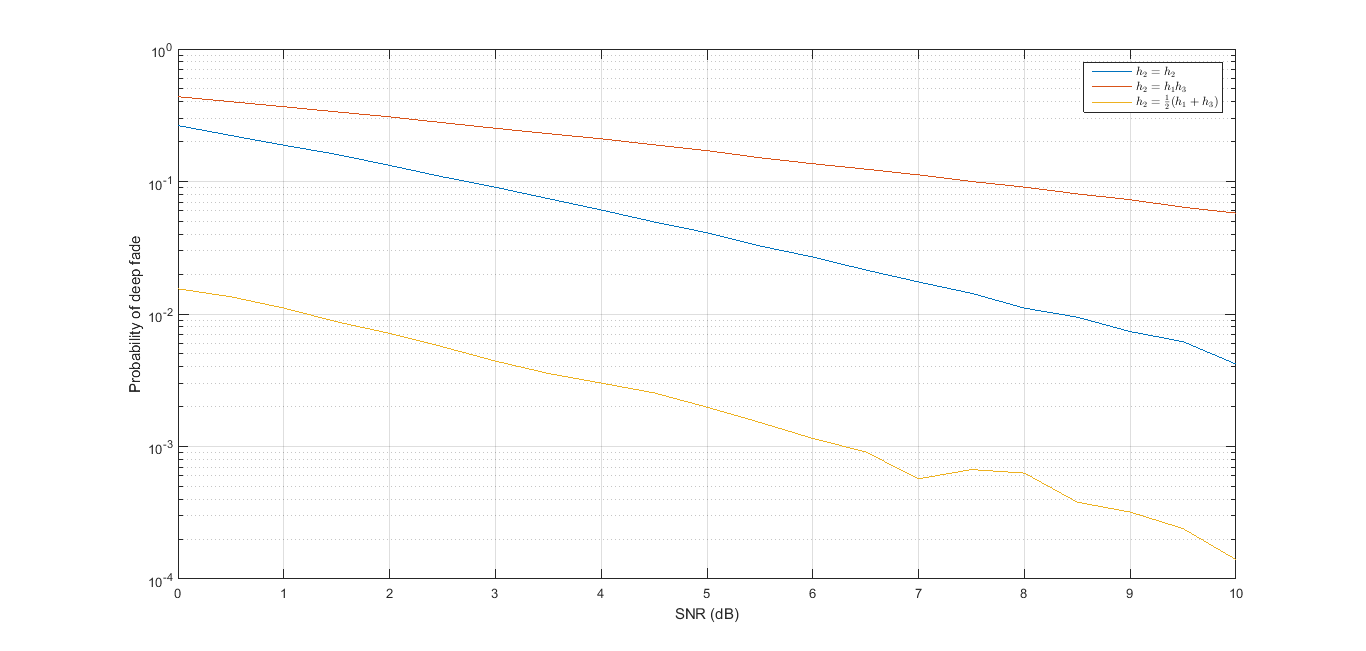
\includegraphics[width=0.9\linewidth]{deepfade01}
\caption{}
\label{fig:deepfade01}
\end{figure}




\section{Problem 3}
\begin{figure}[h!]
\centering
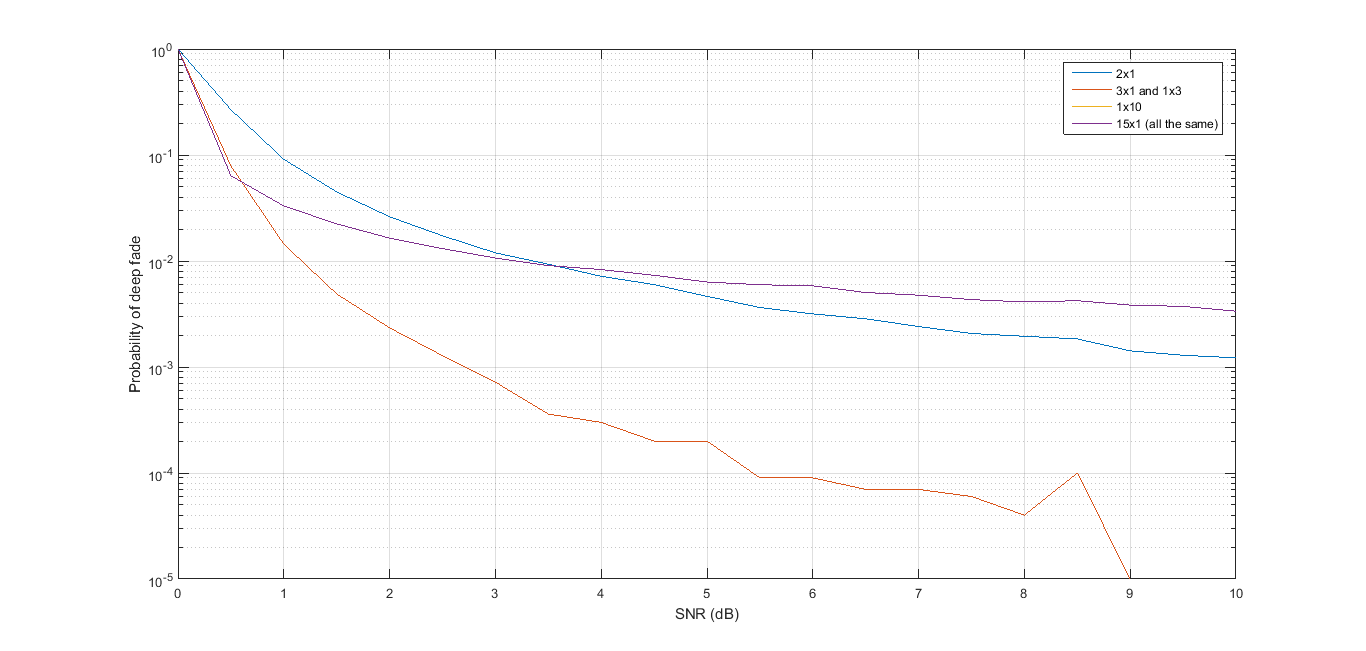
\includegraphics[width=0.9\linewidth]{deepfade02}
\caption{}
\label{fig:deepfade02}
\end{figure}



\section{Problem 4}
We created different experiments to check the validity of some assumptions.

\begin{itemize}
	\item The far tail for the Gaussian random variable \(h_r \sim  \mathcal{N}(0,1) \) is approximated by the exponential \(e^{-x^2/2}\)
	
As we can see in Fig. \ref{fig:problem401} when x is big the complementary cumulative distribution function is very near to the exponential and the difference between them is negligible.
	
\begin{figure}[h!]
\centering
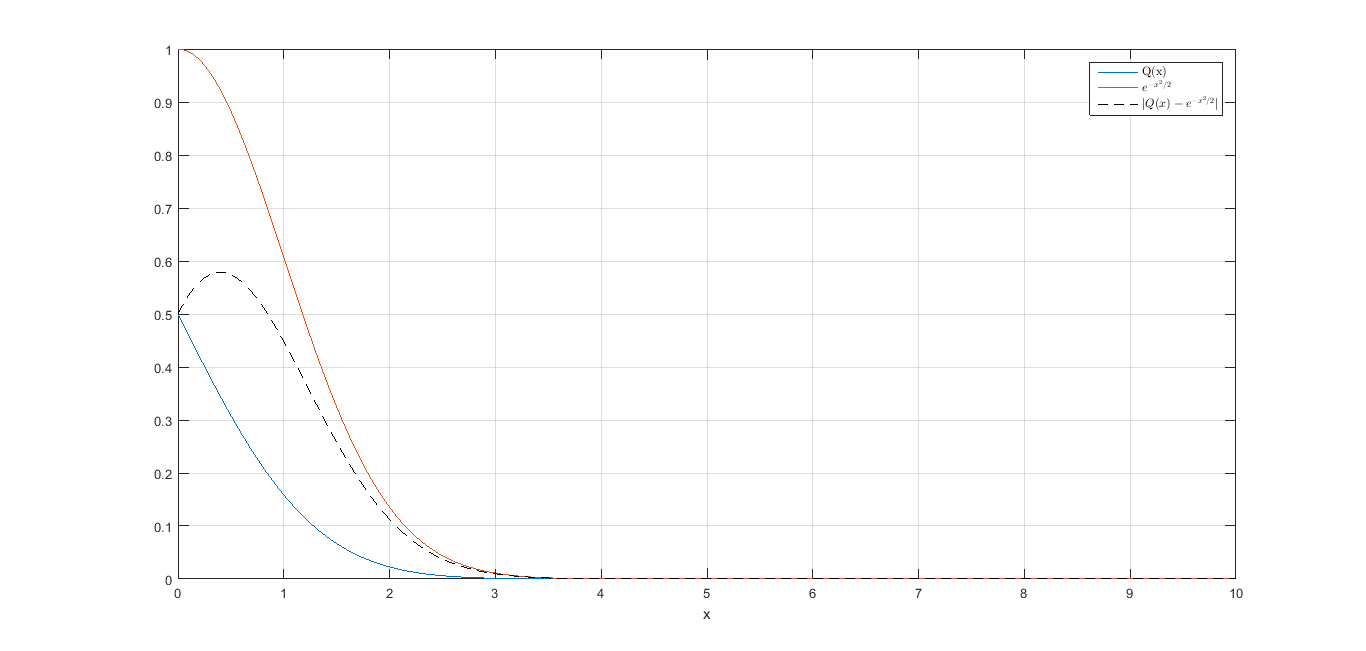
\includegraphics[width=0.9\linewidth]{problem401}
\caption{}
\label{fig:problem401}
\end{figure}

\end{itemize}

\end{document}

